\section{Background}



\subsection{Stable Diffusion}
Stable Diffusion (SD) is a Latent Diffusion Model (LDM) which are used for image generation. LDMs are trained to create a desired image by repeatedly denoising random gaussian noise. What separates LDMs from regular Diffusion Models though is that they apply the diffusion process in a lower-dimensional latent space instead of the pixel-space. This greatly alleviates the need for extensive resources, especially when generating larger images. LDMs have three main components: 1) the autoencoder, 2) the U-Net and 3) the text-encoder.
\begin{figure}[!htb]
\centering
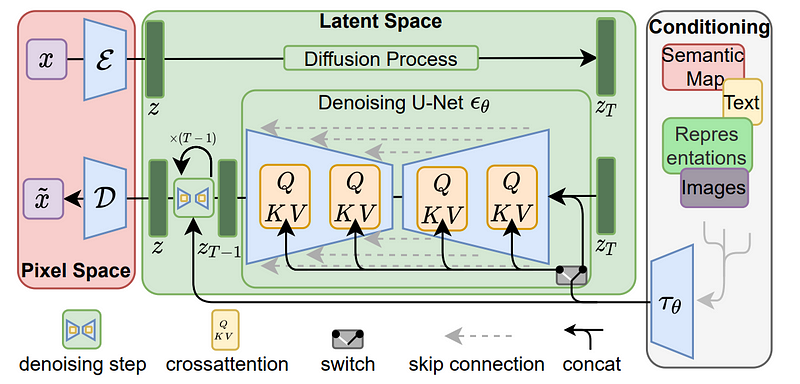
\includegraphics[width=0.8\textwidth]
{static/LDM.png}
\caption{LDM \cite[Fig.~3]{Rombach_2022_CVPR}.}
\label{fig:ldm}
\end{figure}



\subsubsection{The Autoencoder}
A Variational Autoencoder (VAE) consists of two parts: the encoder and the decoder. "During latent diffusion training, the encoder is used to get the latent representations (latents) of the images for the forward diffusion process, which applies more and more noise at each step" \cite{patil2022stable}. The decoder conversely transforms the denoised latents back into an image at the end of the diffusion process. Only the decoder is used for the image generation process.



\subsubsection{The U-Net}
The U-Net is type of Convolutional Neural Network (CNN) that is responsible for computing the expected noise of every image in every diffusion step. This expected noise is slowly removed from the image to get closer to the desired output with every denoising step. It's called a U-Net because it itself has an encoder and a decoder with transformer-based blocks. "It first encodes the current
noised image as a set of tokens, then passes it through a
series of transformer blocks" \cite{bolya2023tomesd}. Another thing that seperates a U-Net from an autoencoder are the skip connections that directly pass information from the encoder to the decoder, aiding in the preservation of details during upsampling (see Fig.~\ref{fig:ldm}). Every transformer block has a self attention (self-attn), cross attention (cross-attn) and multi-layer perceptron (mlp) module.



\subsubsection{Transformer Architecture}
Different components: Self-Attention (self-attn), Cross-Attention (cross-attn) and Multi-Layer Perceptron (mlp).



\subsubsection{Attention and Self-Attention}
Text.



\subsubsection{The Text-Encoder}
Text.



\subsubsection{Training?}
Forward diffusion. Noise is added to an image. NN trained on it.



\subsection{Frechet-Inception-Distance (FID)}
PyTorch implementation\cite{Seitzer2020FID}



\subsubsection{Inception Model}
Text.




\subsubsection{Caveats}
Inception model is biased. Inception model compresses images to 299x299 pixels. FID inconsistent with ToMe applied (not exactly reproducable)



\subsection{What are Tokens?}
In image synthesis, a token is a block of pixels that are processed collectively by the transformer. Stable Diffusion uses the CLIP tokenizer \cite{radford2021learning} which defines a token as an $14 \times 14$ block of pixels. ---CLIP is trained with the ViT-L/14 model---